\documentclass[13pt,oneside]{book}
\usepackage[utf8]{inputenc}
\usepackage{url}
\usepackage{graphicx}

\usepackage{geometry}
\geometry{a4paper, left=20mm, right=20mm, top=20mm, bottom=20mm}
\usepackage{lipsum}
\usepackage{caption}

\begin{document}
\setlipsumdefault{1}

\begin{titlepage}
\begin{center}
{\LARGE College Of Engineering Trivandrum}\\[0.5cm]
{\LARGE Lab Exam Report}\\[2pt]
\linespread{1.2}\huge {\bfseries Application Software Development Lab}\\[3cm]
\linespread{1}

\includegraphics[width=5cm]{img/emblem.jpeg}\\[3cm]
{\Large GOKUL K\\ S5  CSE \\ Roll No:21\\ TVE18CS021 }\\[1cm]


\textit{ }\\[2cm]
Department of Computer Science\\[0.2cm]
\today
\end{center}

\end{titlepage}

\newpage

\begin{frame}{}
    \centering
    \hspace*{-0.5cm}
    $\vcenter{\hbox{
\includegraphics[width=1.5cm]{img/emblem.jpeg}}}$
    $\vcenter{\resizebox{0.95\textwidth}{!}{
        \begin{tabular}{c}
             CS333 - Application Software Development Lab $\cdot$ 2020 $\cdot$   \\
             \hline 
        \end{tabular}
    }}$
\end{frame}

\section*{Questions}
\begin{itemize}
\item 
Create and populate shown tables. Add the following constraints after table creation. \\
a. Song\_ID should be of the format “ID0 " \\
b. Album\_ID should be of the format “AL0 ”, \\
c. Album\_ID should be of the format “AL0 ”, \\
d. Artist\_ID should be of the format “AR0 ”. \\
\begin{verbatim}
	CREATE TABLE Song (
	Song_ID VARCHAR(20) PRIMARY KEY,
	Song_Name VARCHAR(20),
	Album_ID VARCHAR(20),
	Genre VARCHAR(20),
	Views INTEGER,
	FOREIGN KEY (Album_ID) REFERENCES Album(Album_ID)
);

CREATE TABLE Album (
	Album_ID VARCHAR(20) PRIMARY KEY,
	Album_Name VARCHAR(20),
	Artist_ID VARCHAR(20),
	Release_Date DATE,
	Sales INTEGER,
	FOREIGN KEY (Artist_ID) REFERENCES Artist(Artist_ID)
);

CREATE TABLE Artist (
	Artist_ID VARCHAR(20) PRIMARY KEY,
	Artist_Name VARCHAR(20),
	Country VARCHAR(20)
);

CREATE TABLE Grammy (
	Year INTEGER,
	Song_ID VARCHAR(20),
	PRIMARY KEY (Year, Song_ID),
	FOREIGN KEY (Song_ID) REFERENCES Song(Song_ID)
);

ALTER TABLE Song
ADD CONSTRAINT song_id_format CHECK (Song_ID LIKE 'ID0%');

ALTER TABLE Album
ADD CONSTRAINT album_id_format CHECK (Album_ID LIKE 'AL0%');

ALTER TABLE Artist
ADD CONSTRAINT album_id_format CHECK (Artist_ID LIKE 'AR0%');
\end{verbatim}
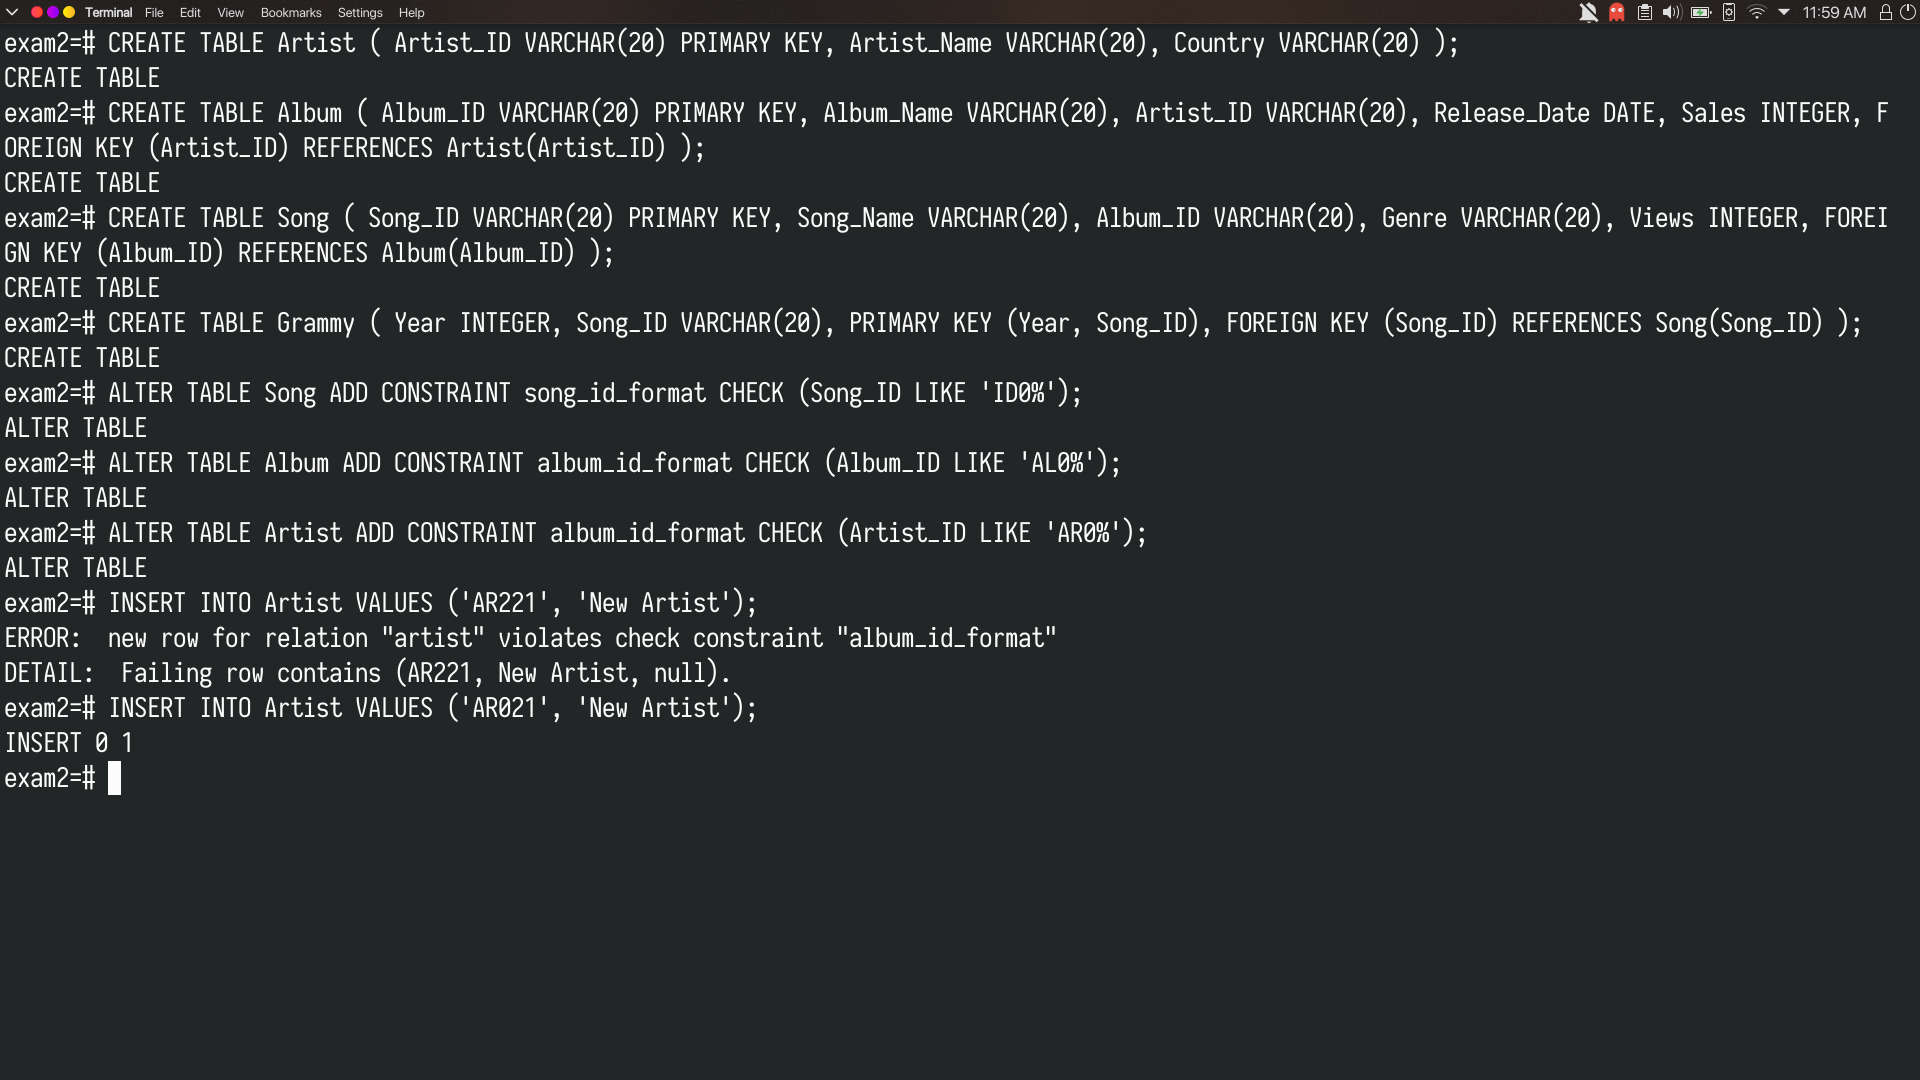
\includegraphics[width=\textwidth]{img/q/1_constraintcheck.png}

\begin{verbatim}
    
INSERT INTO Song VALUES ('ID001', 'Panic', 'AL004', 'Pop', 650),
	('ID002', 'Dignity', 'AL001', 'Rap', 1900),
	('ID003', 'Expressed', 'AL002', 'Pop', 1500),
	('ID004', 'Science', 'AL005', 'Rock', 1920),
	('ID005', 'Illusion', 'AL003', 'Rock', 760),
	('ID006', 'Bomber', 'AL002', 'Rap', 2000),
	('ID007', 'Agenda', 'AL004', 'Jazz', 1260),
	('ID008', 'River', 'AL002', 'Pop', 920);

INSERT INTO Album VALUES ('AL001', 'Jurisdiction', 'AR004', '2004-03-16', 570),
	('AL002', 'Limitless', 'AR003', '2006-05-24', 650),
	('AL003', '69 cents', 'AR001', '2005-09-06', 400),
	('AL004', 'Confession', 'AR002', '2012-11-28', 120),	
	('AL005', 'Hero', 'AR004', '2002-07-07', 900);	

INSERT INTO Artist VALUES ('AR001', 'Natalia', 'France'),
	('AR002', 'Suman', 'India'),
	('AR003', 'Hill', 'USA'),
	('AR004', 'Sham', 'France');
	


INSERT INTO Grammy VALUES (2003, 'ID004'),
	(2007, 'ID006'),
	(2009, 'ID003'),
	(2004, 'ID002'),
	(2012, 'ID007');

\end{verbatim}

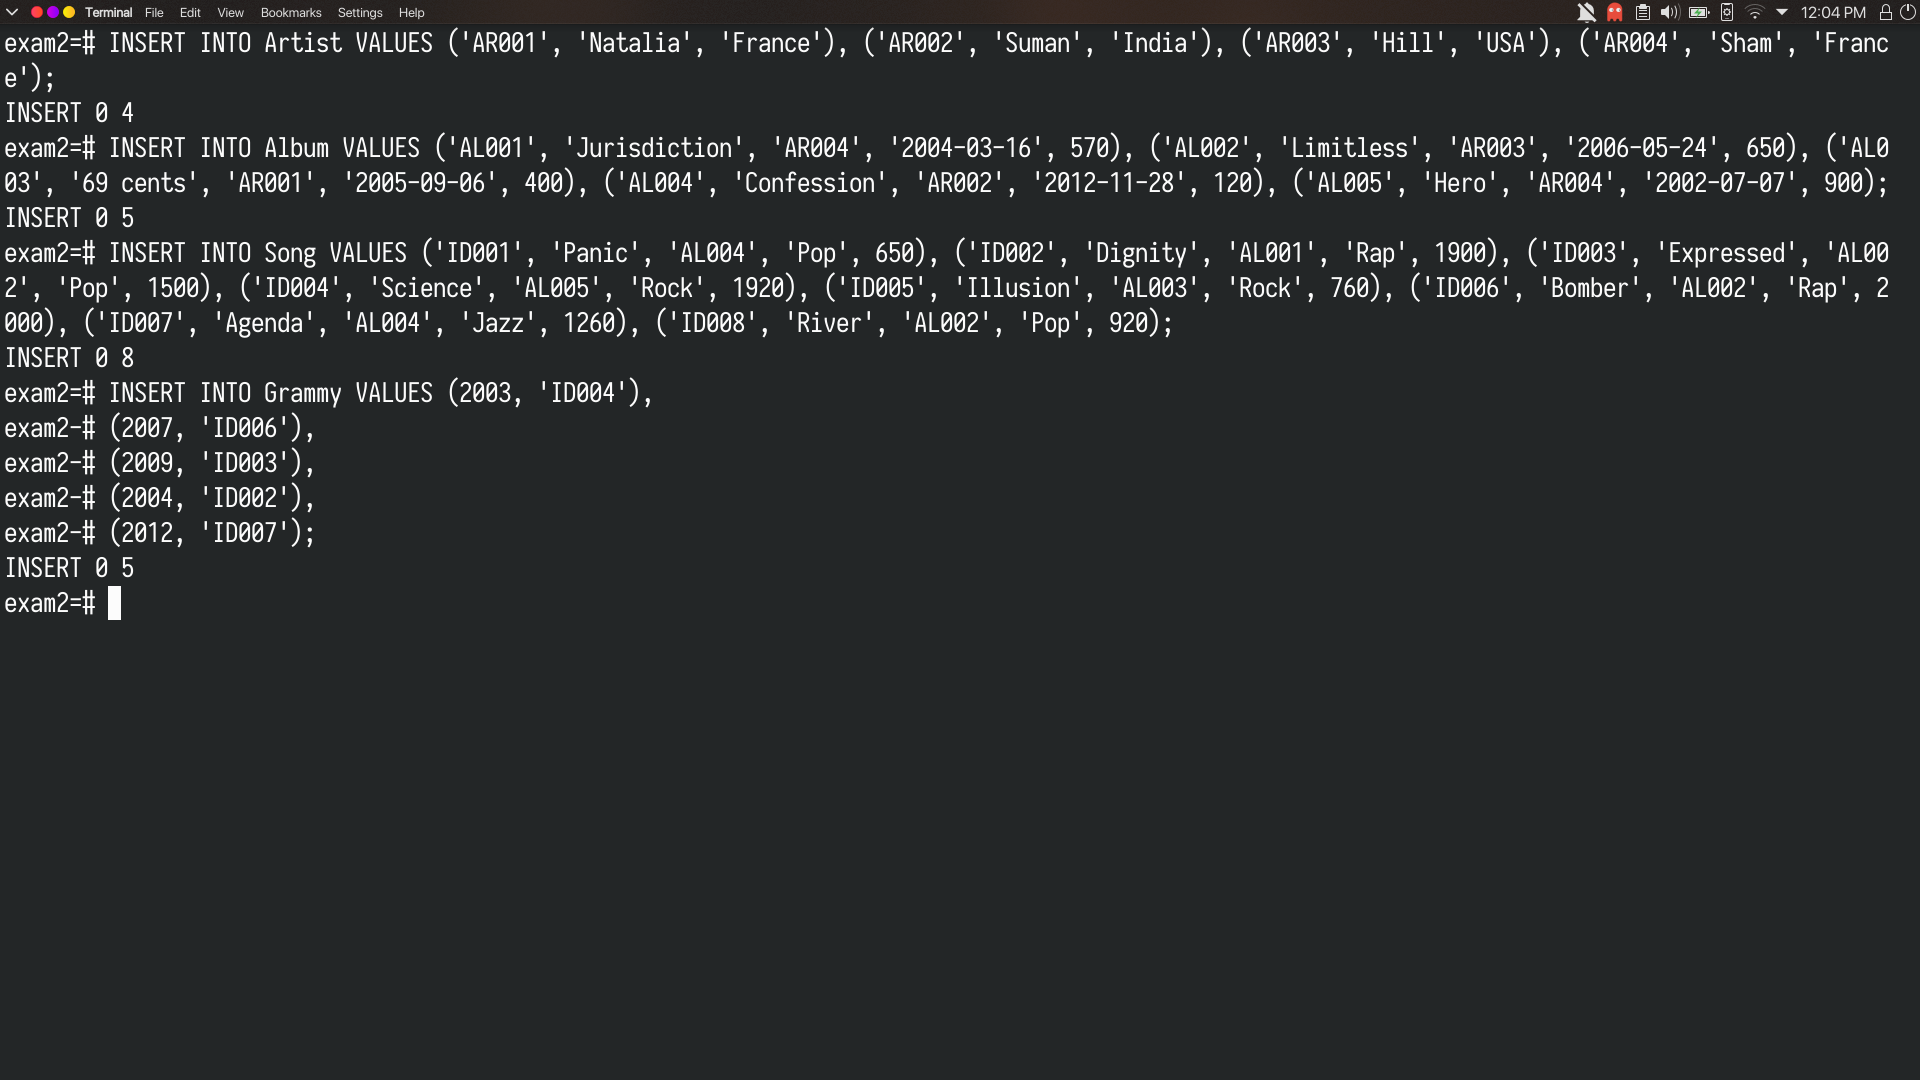
\includegraphics[width=\textwidth]{img/q/2_insertion.png}

\item
List all the songs by Hill released after 2005.
 
Syntax:
\begin{verbatim}
SELECT * FROM Song 
WHERE Album_ID IN 
    (SELECT Album_ID FROM Album 
    WHERE Artist_ID=(
        SELECT Artist_ID FROM Artist 
        WHERE Artist_Name='Hill') 
    AND Release_Date >= '2006-01-01'
    );
\end{verbatim}
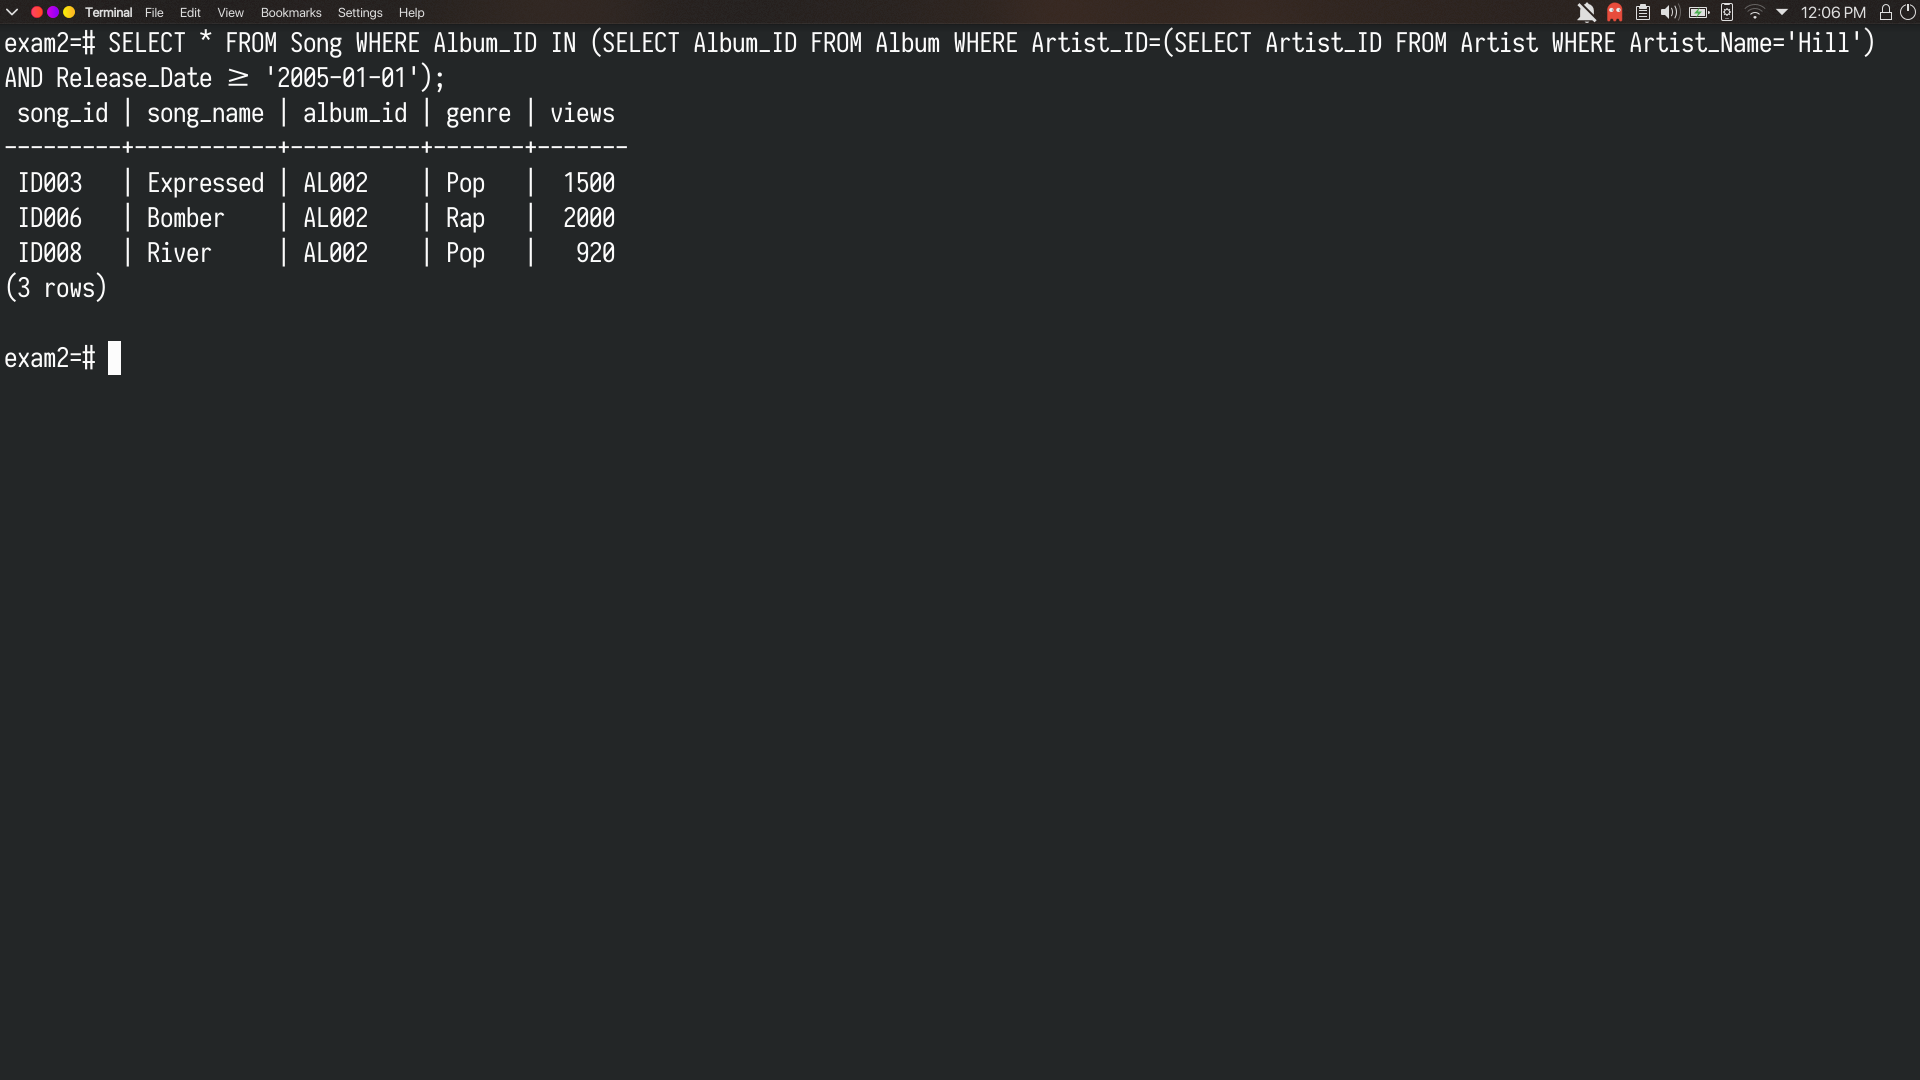
\includegraphics[width=\textwidth]{img/q/2.png}


\item
List all songs in the same album as Bomber.
 
Syntax:
\begin{verbatim}
SELECT * FROM Song 
WHERE Album_ID = 
    (SELECT Album_ID FROM Song 
    WHERE Song_Name = 'Bomber');

\end{verbatim}
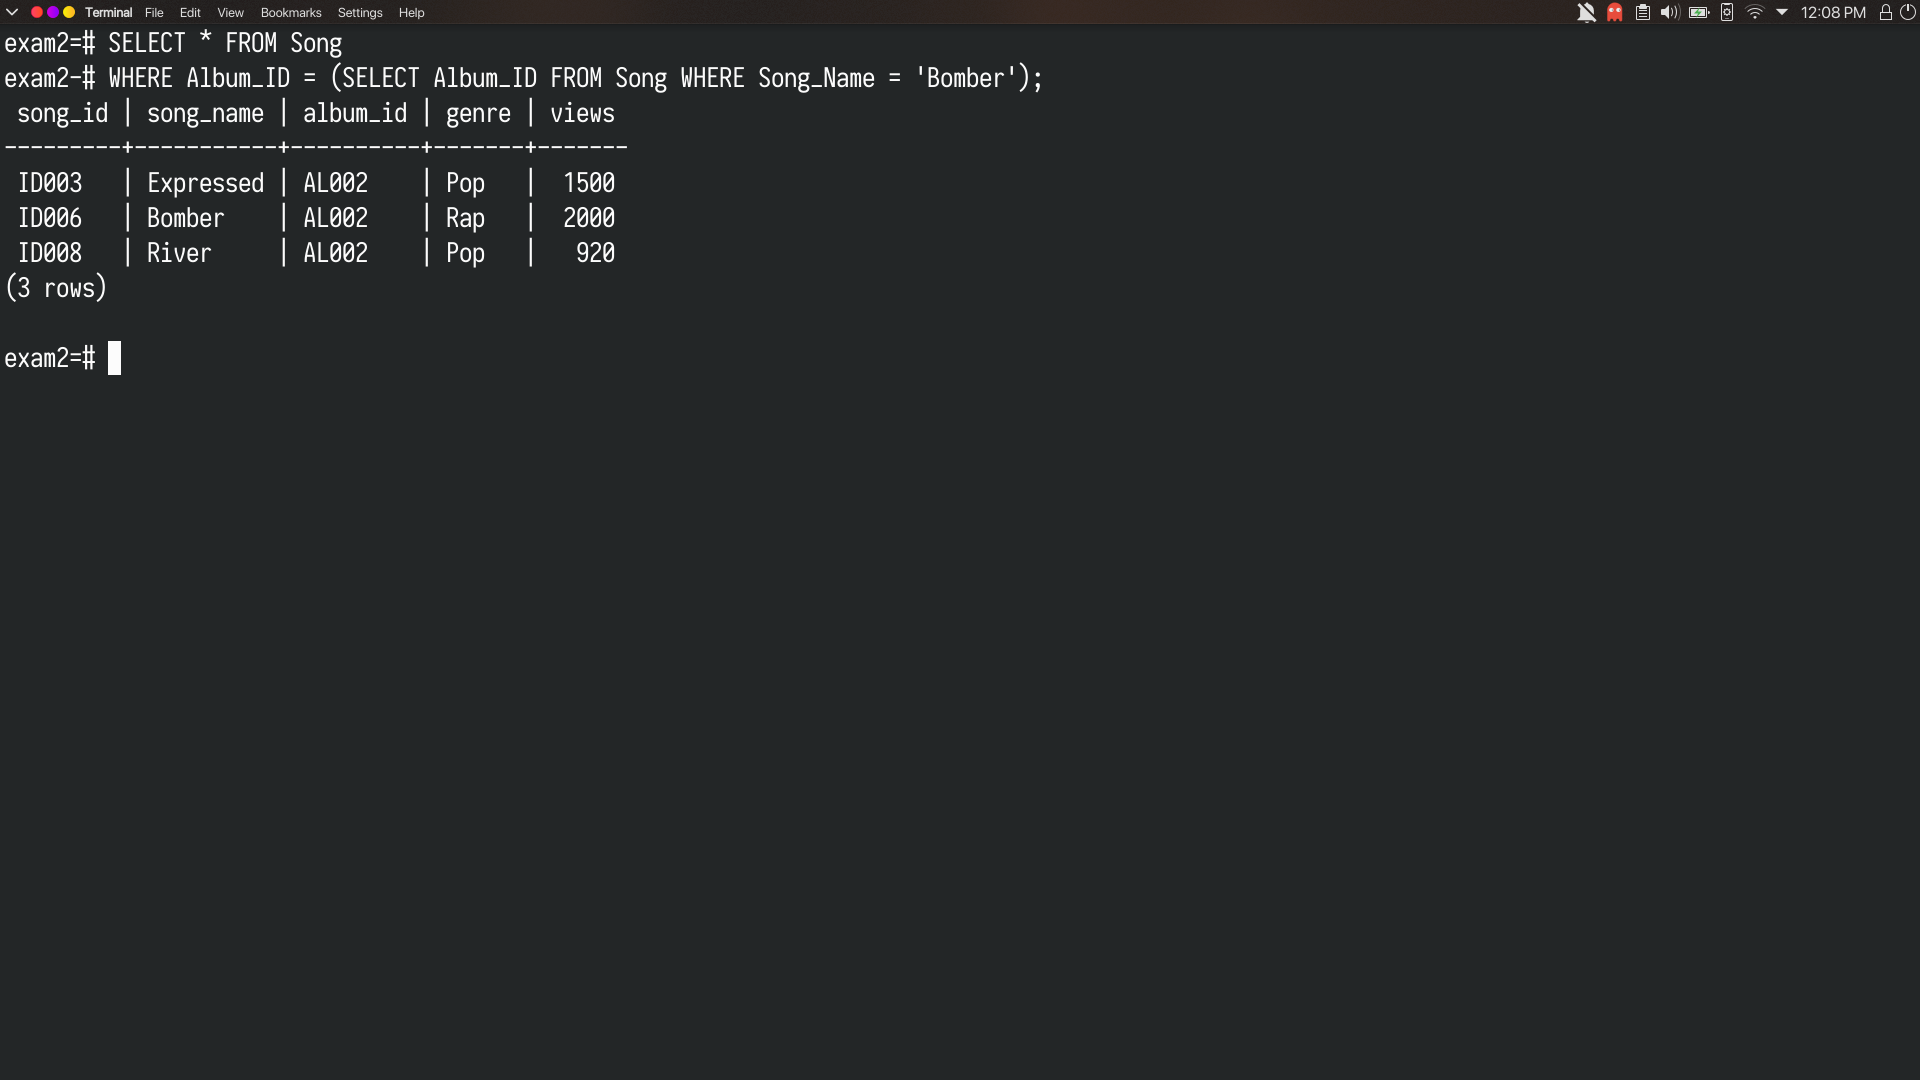
\includegraphics[width=\textwidth]{img/q/3.png}


\item
Find the total number of views of all albums with sales more than 350
 
Syntax:
\begin{verbatim}
SELECT SUM(s.views) 
FROM Song s, Album a
WHERE a.Sales > 350 AND a.Album_ID = s.Album_ID;

\end{verbatim}
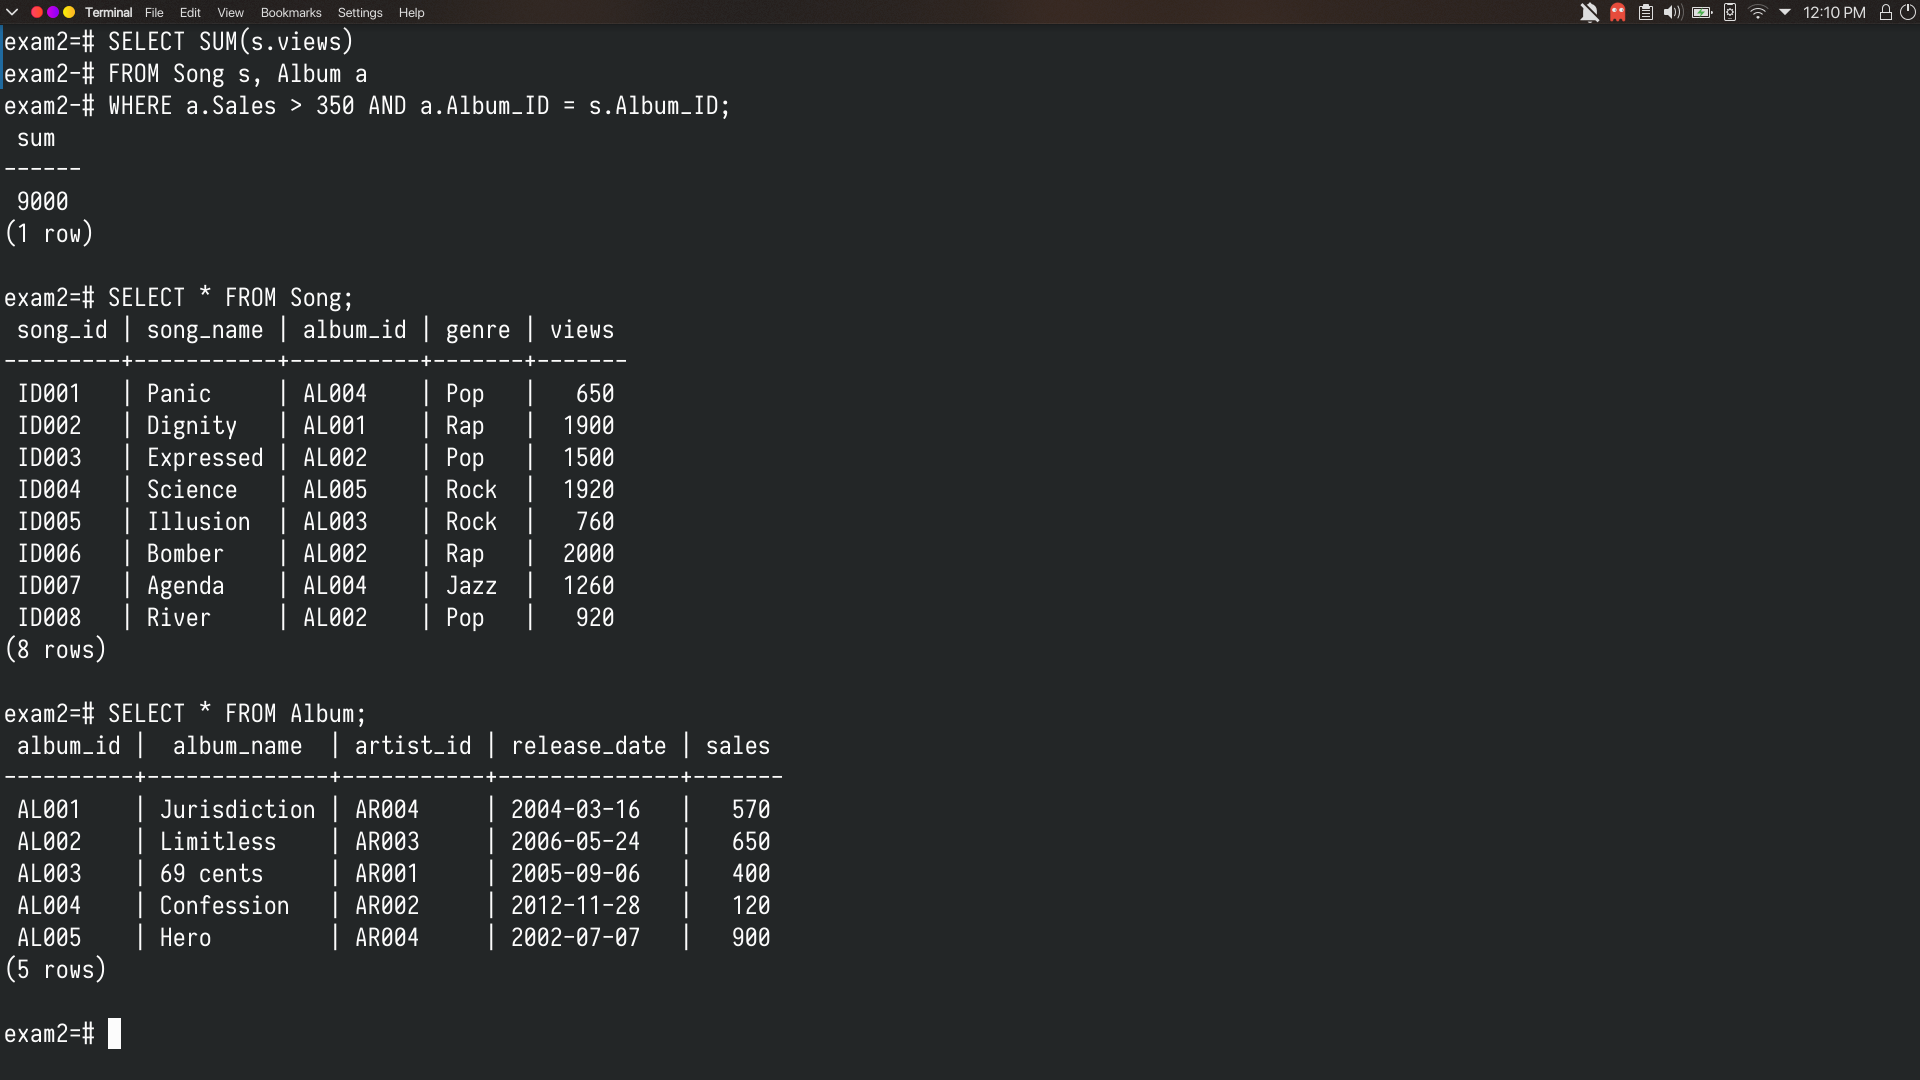
\includegraphics[width=\textwidth]{img/q/4.png}

\item
List the number of songs that didn't win a Grammy in each album
 
Syntax:
\begin{verbatim}
SELECT a.Album_Name, COUNT(*)
FROM Song s, Album a
WHERE a.Album_ID = s.Album_ID AND s.Song_ID NOT IN (Select Song_ID FROM Grammy)
GROUP BY a.Album_Name;
\end{verbatim}
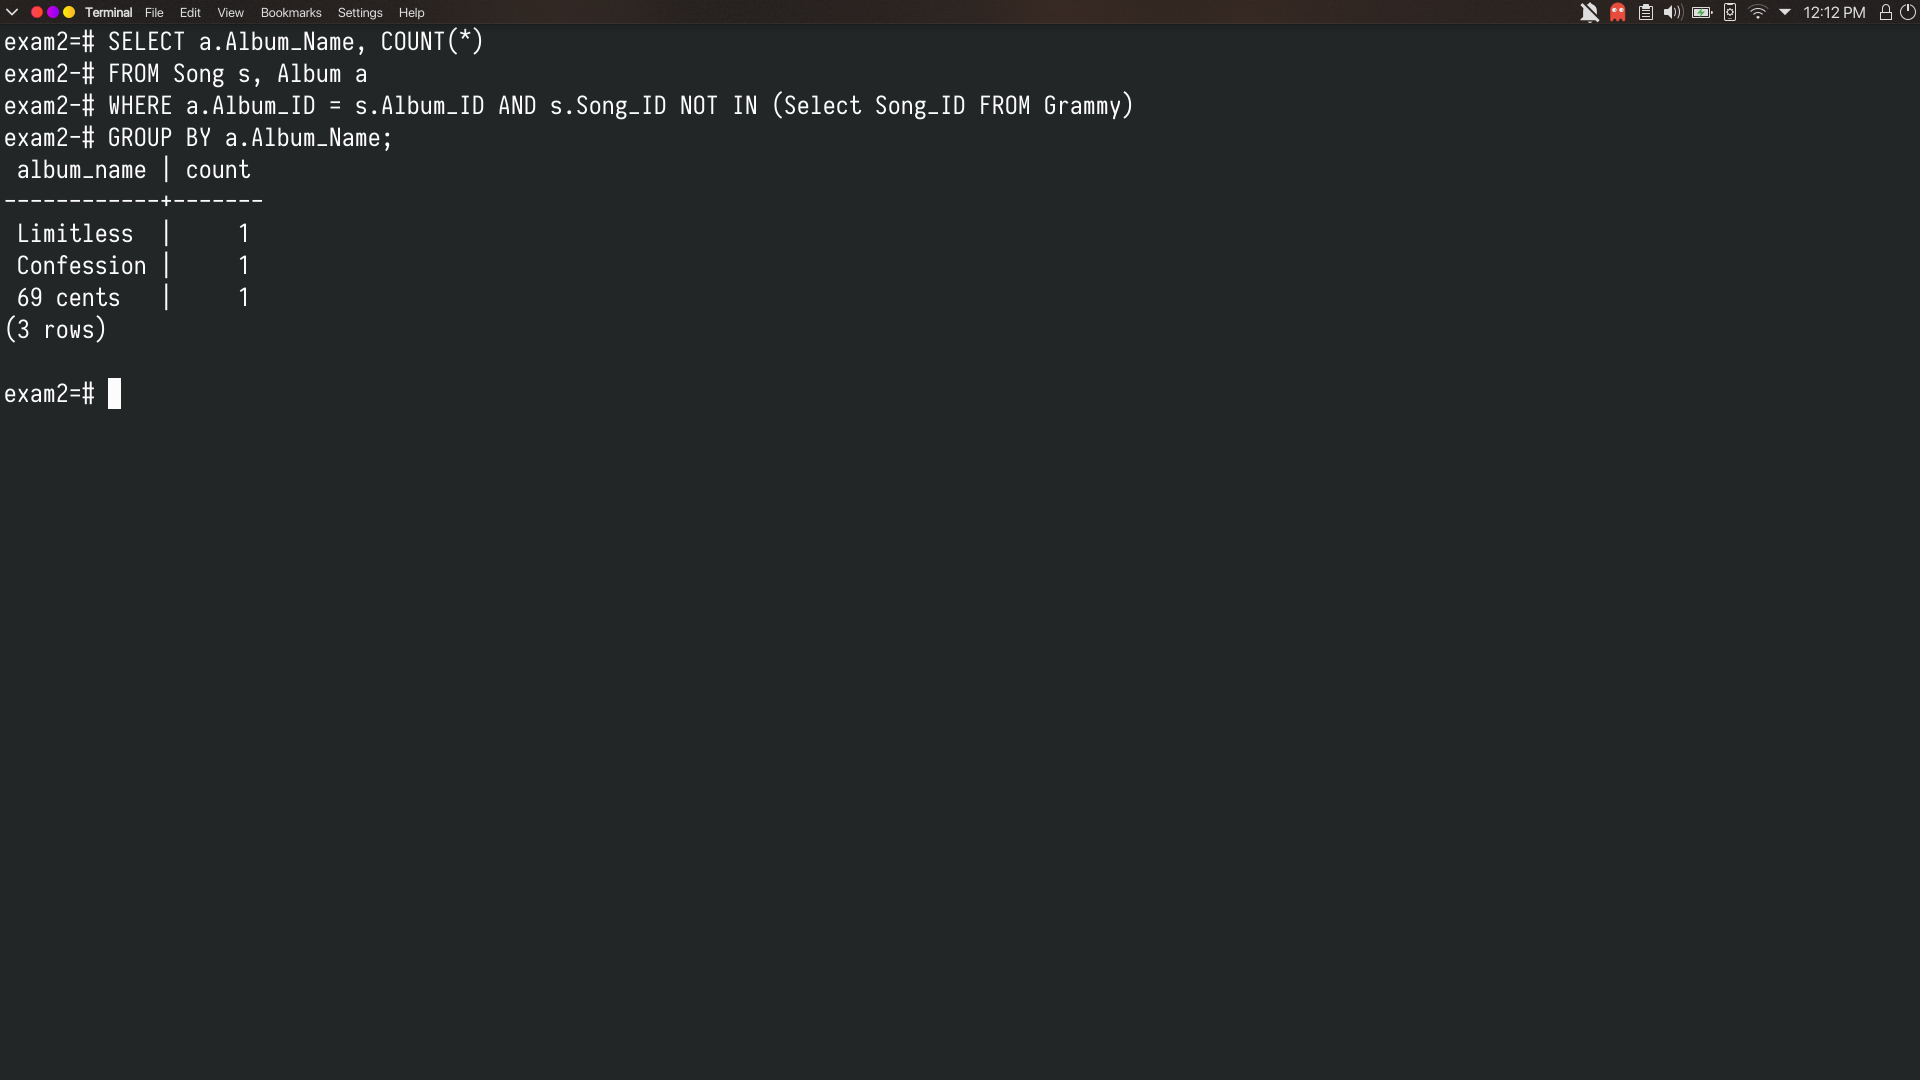
\includegraphics[width=\textwidth]{img/q/5.png}


\item
Create a Trigger such that whenever a new song is added, if it has more than 1000 views,
it wins a Grammy in that year itself.
 
Syntax:
\begin{verbatim}
CREATE OR REPLACE FUNCTION fn_grammy_check() RETURNS TRIGGER AS
$grammy_proc$
	DECLARE
		year INT;
	BEGIN
		IF NEW.Views > 1000
		THEN
			year = (SELECT TO_CHAR(Album.Release_Date, 'YYYY') 
			FROM Album 
			WHERE Album_ID = NEW.Album_ID);
			INSERT INTO Grammy VALUES (year, New.Song_ID);
			RAISE INFO 'inserted';
		END IF;
		RETURN NEW;
	END;
$grammy_proc$
LANGUAGE plpgsql;

CREATE TRIGGER grammy_trigger
AFTER INSERT ON Song
	FOR EACH ROW EXECUTE PROCEDURE grammy_proc();


\end{verbatim}
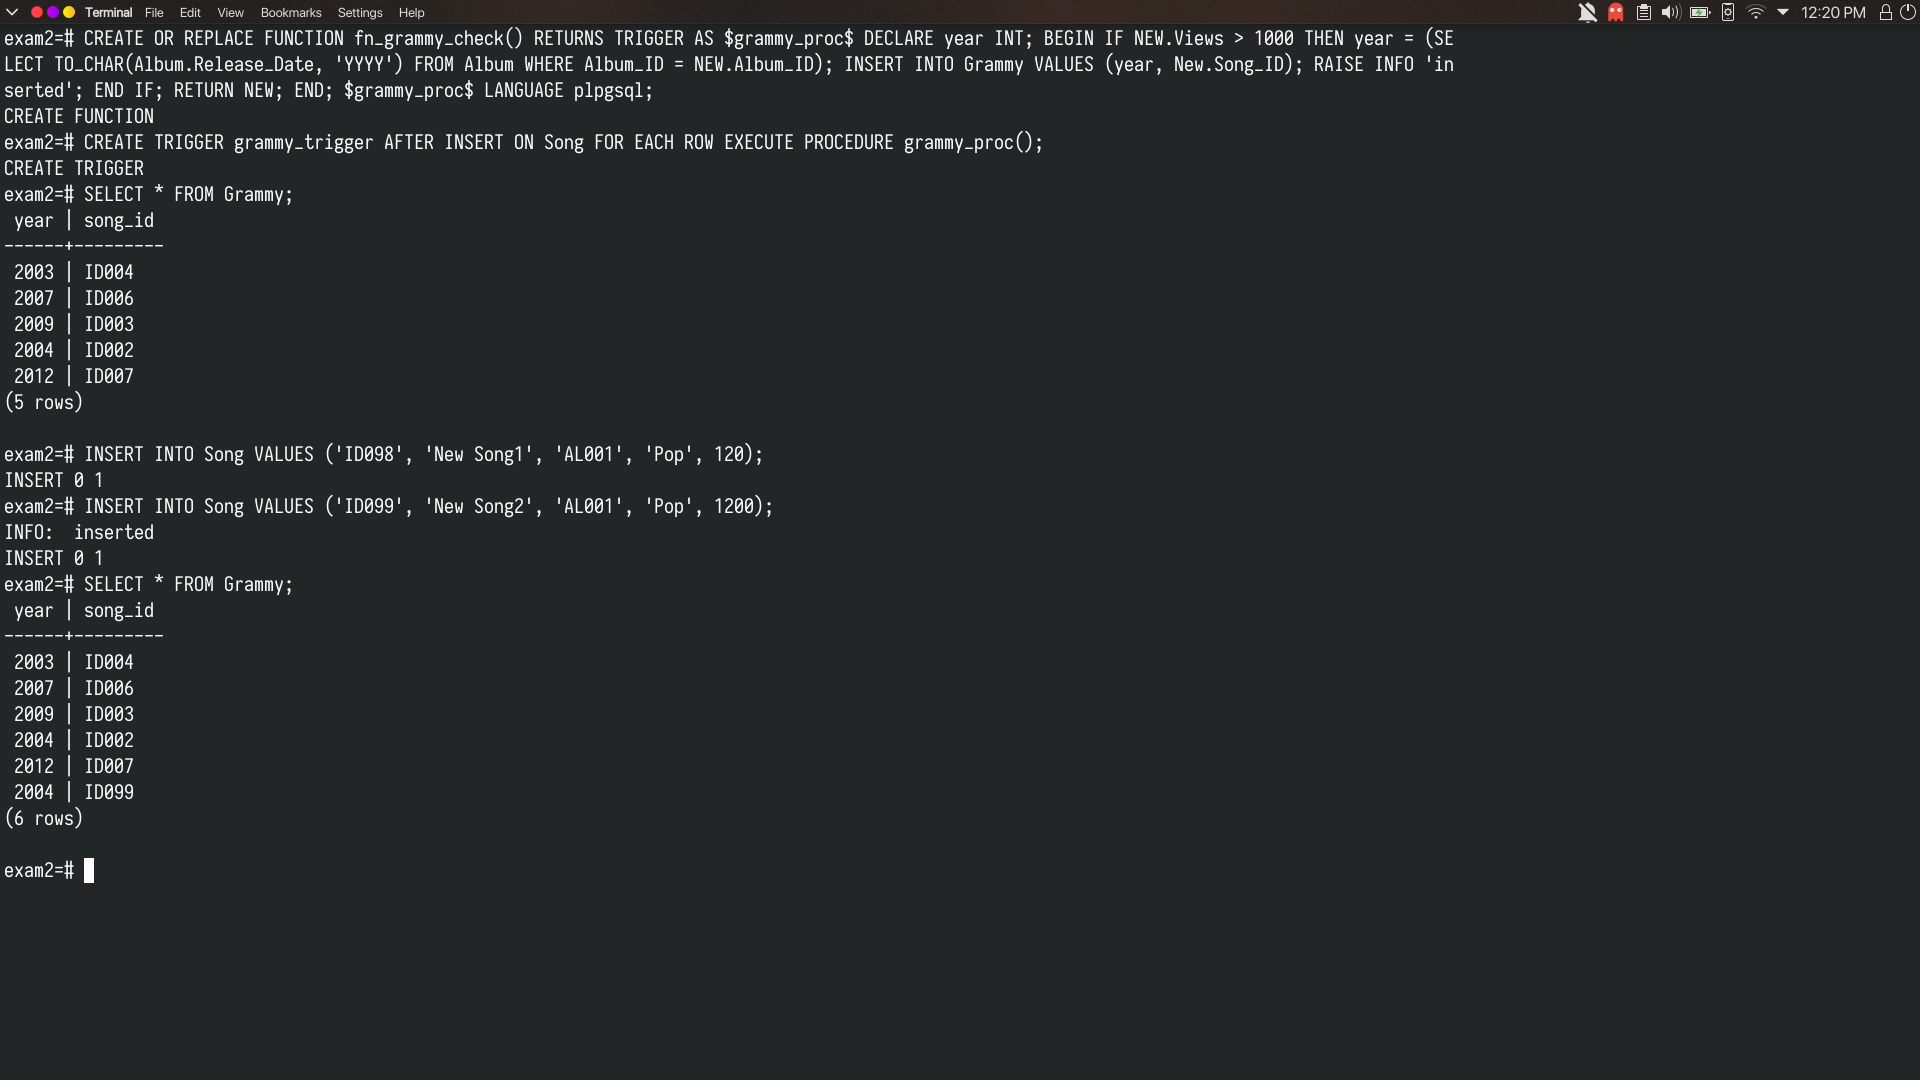
\includegraphics[width=\textwidth]{img/q/6.png}


\item
Create a view “Grammy Winners” which contains the name of the song, album and artists
which won the Grammy on the year they released.

Syntax:
\begin{verbatim}
CREATE OR REPLACE VIEW grammy_winners AS SELECT s.Song_Name, a.Album_Name, ar.Artist_Name
FROM Song s, Album a, Artist ar, Grammy g
WHERE s.Album_ID = a.Album_ID AND ar.Artist_ID = a.Artist_ID AND g.Song_ID = s.Song_ID
AND g.Year = CAST(TO_CHAR(a.Release_Date, 'YYYY') AS INTEGER);
\end{verbatim}
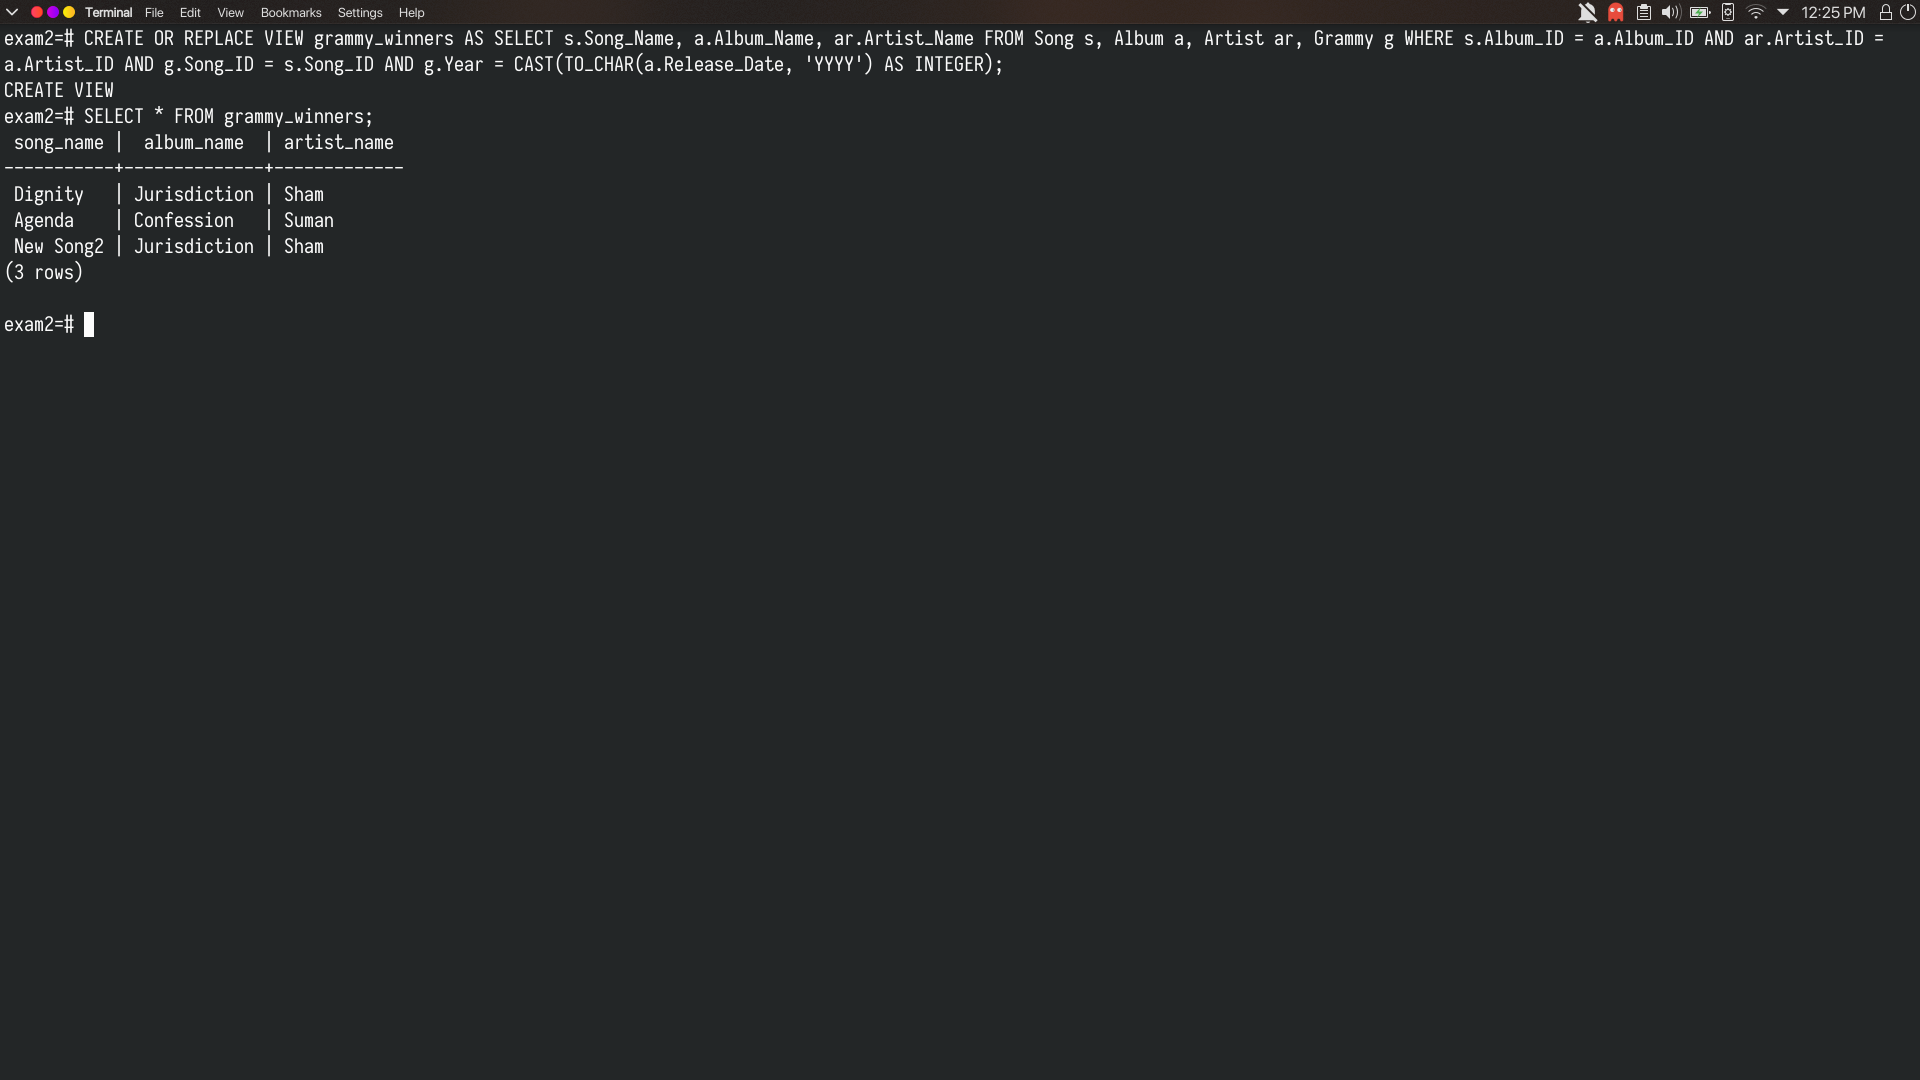
\includegraphics[width=\textwidth]{img/q/7.png}


\item
Use a cursor to increase the sales by 5\% for all albums released after 2010.
 
Syntax:
\begin{verbatim}
CREATE OR REPLACE FUNCTION increase_sales()
RETURNS VOID AS $$
DECLARE
	albumr RECORD;
	album_cursor CURSOR FOR Select * FROM Album;
BEGIN
	OPEN album_cursor;
	LOOP
		FETCH album_cursor INTO albumr;
		EXIT WHEN NOT FOUND;
		IF TO_CHAR(albumr.Release_Date, 'YYYY') > '2010'
		THEN
			UPDATE Album SET Sales = sales * 1.05 WHERE Album_ID = albumr.Album_ID;
			RAISE INFO 'Updating';
		END IF;
	END LOOP;
	CLOSE album_cursor;
END;
$$ LANGUAGE plpgsql;

\end{verbatim}
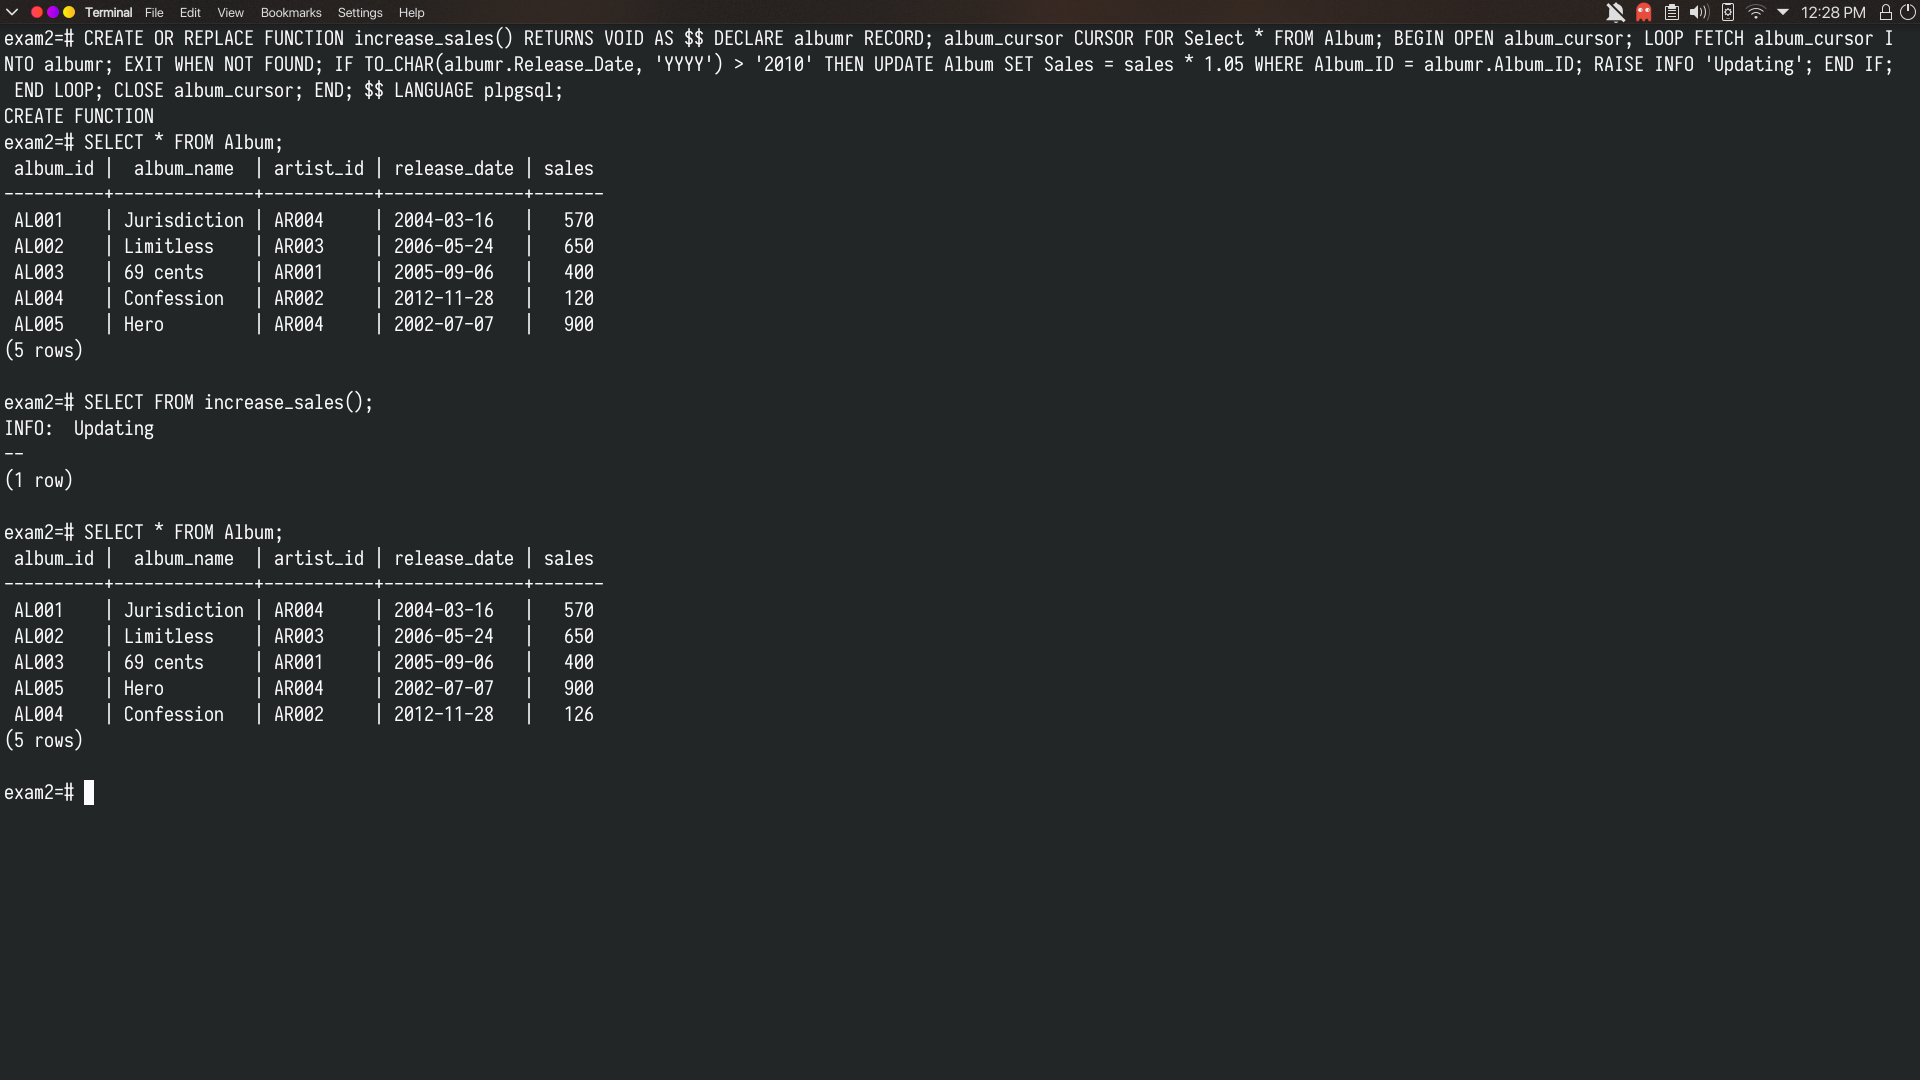
\includegraphics[width=\textwidth]{img/q/8.png}


\item
Create a package (or schema) consisting of the following functions and procedures:
1. For the above database, write a function to multiply the sales value of all
albums which have received a Grammy award with the number of Grammys
received and update the sales column.
2. Write a procedure to display the Genre of music that has received most
Grammys
 
Syntax:
\begin{verbatim}
CREATE SCHEMA sc1;
CREATE OR REPLACE FUNCTION sc1.func_grammy_sales() RETURNS VOID AS $$
DECLARE
	album_cursor CURSOR FOR SELECT * FROM Album;
	album_record RECORD;
	grammy_wins INT;
BEGIN
	OPEN album_cursor;
	loop
	  FETCH album_cursor INTO album_record;
	  EXIT WHEN NOT FOUND;
		grammy_wins = (SELECT COUNT(s.Song_ID) FROM Song s, Grammy g 
		    WHERE s.Album_ID = album_record.Album_ID AND g.Song_ID = s.Song_ID);
		UPDATE Album SET sales = sales * COALESCE(NULLIF(grammy_wins, 0), 1) 
		WHERE Album_ID = album_record.Album_ID;
	end loop;
	CLOSE album_cursor;
END;
$$ LANGUAGE plpgsql;
CREATE OR REPLACE PROCEDURE sc1.grammy_genre() 
LANGUAGE plpgsql AS $$
DECLARE
	genre VARCHAR(10);
BEGIN
	genre = ( SELECT s.Genre FROM Album a, Song s, Grammy g 
	WHERE a.Album_ID = s.Album_ID AND g.Song_ID = s.Song_ID 
	GROUP BY s.Genre 
	ORDER BY COUNT(s.Genre) DESC 
	LIMIT 1);
	RAISE INFO 'The genre is %', genre;
END;
$$;

\end{verbatim}
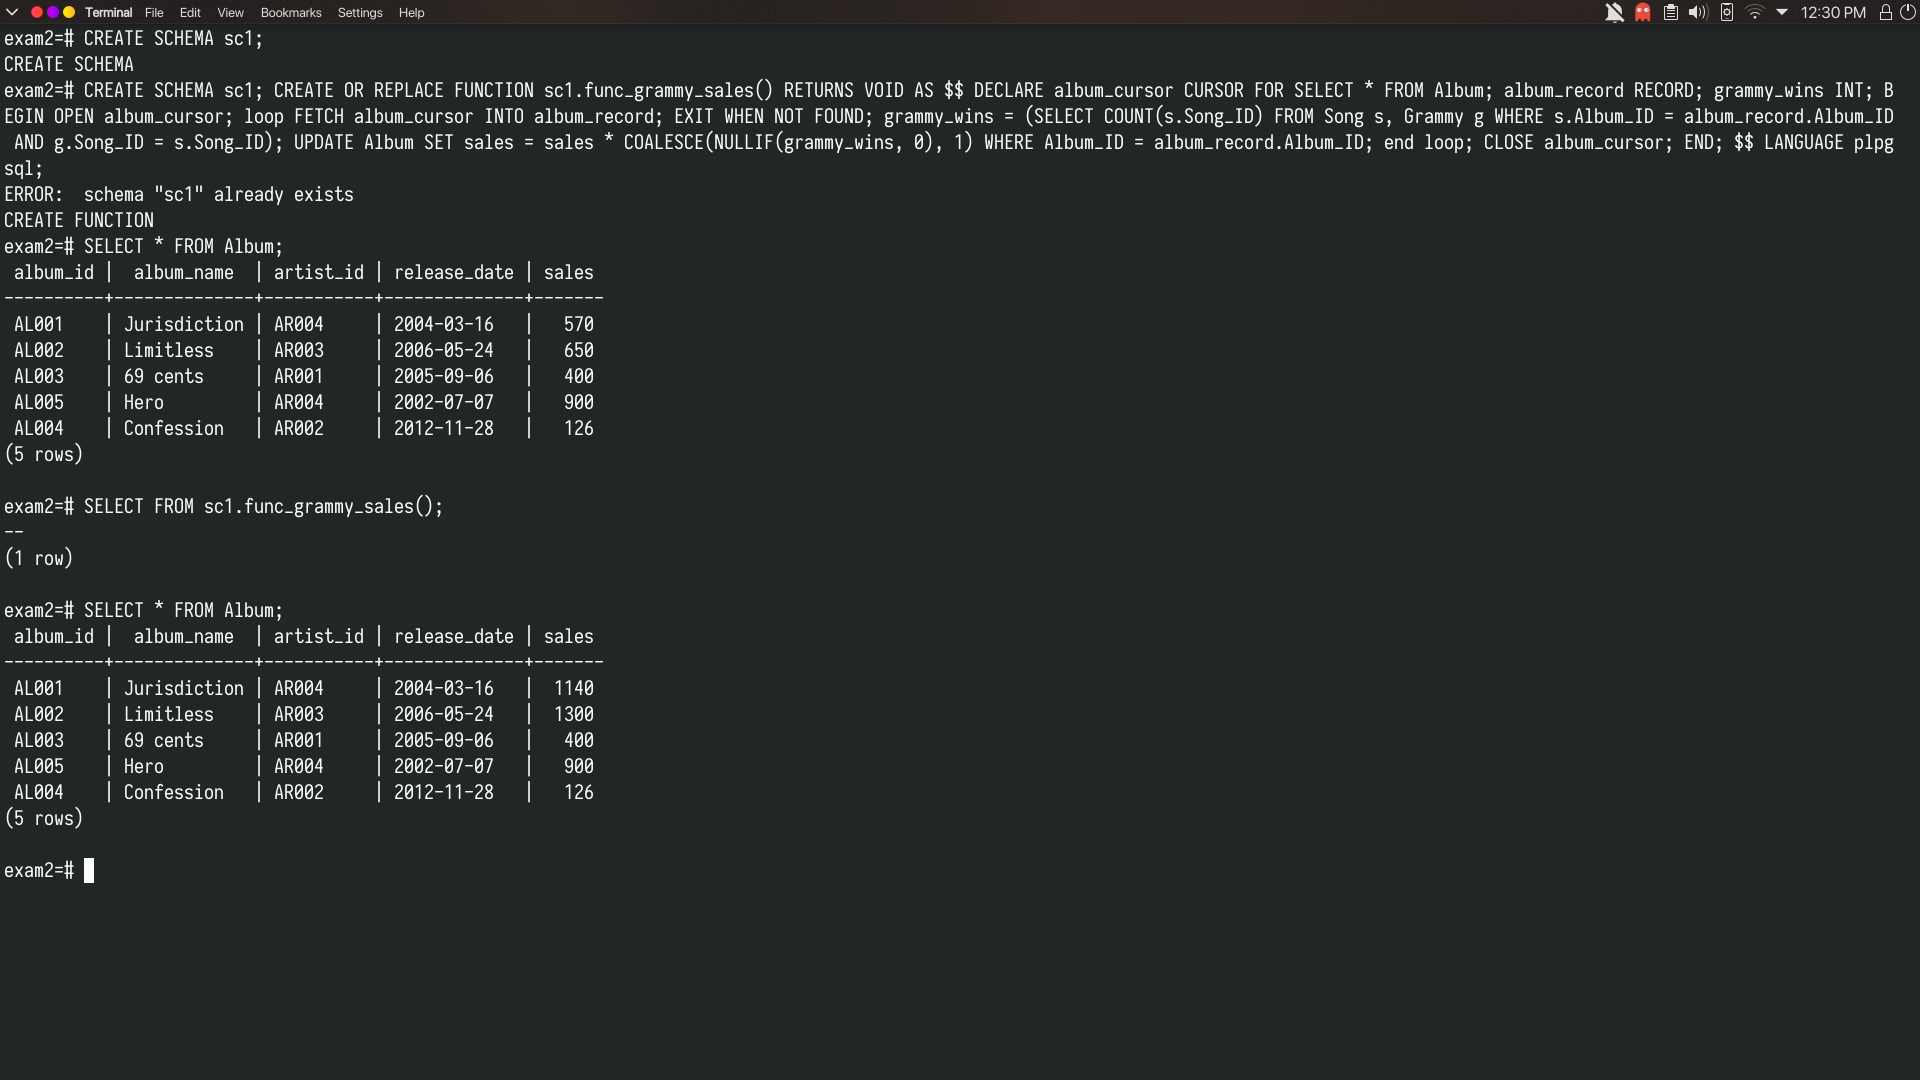
\includegraphics[width=\textwidth]{img/q/9.png}
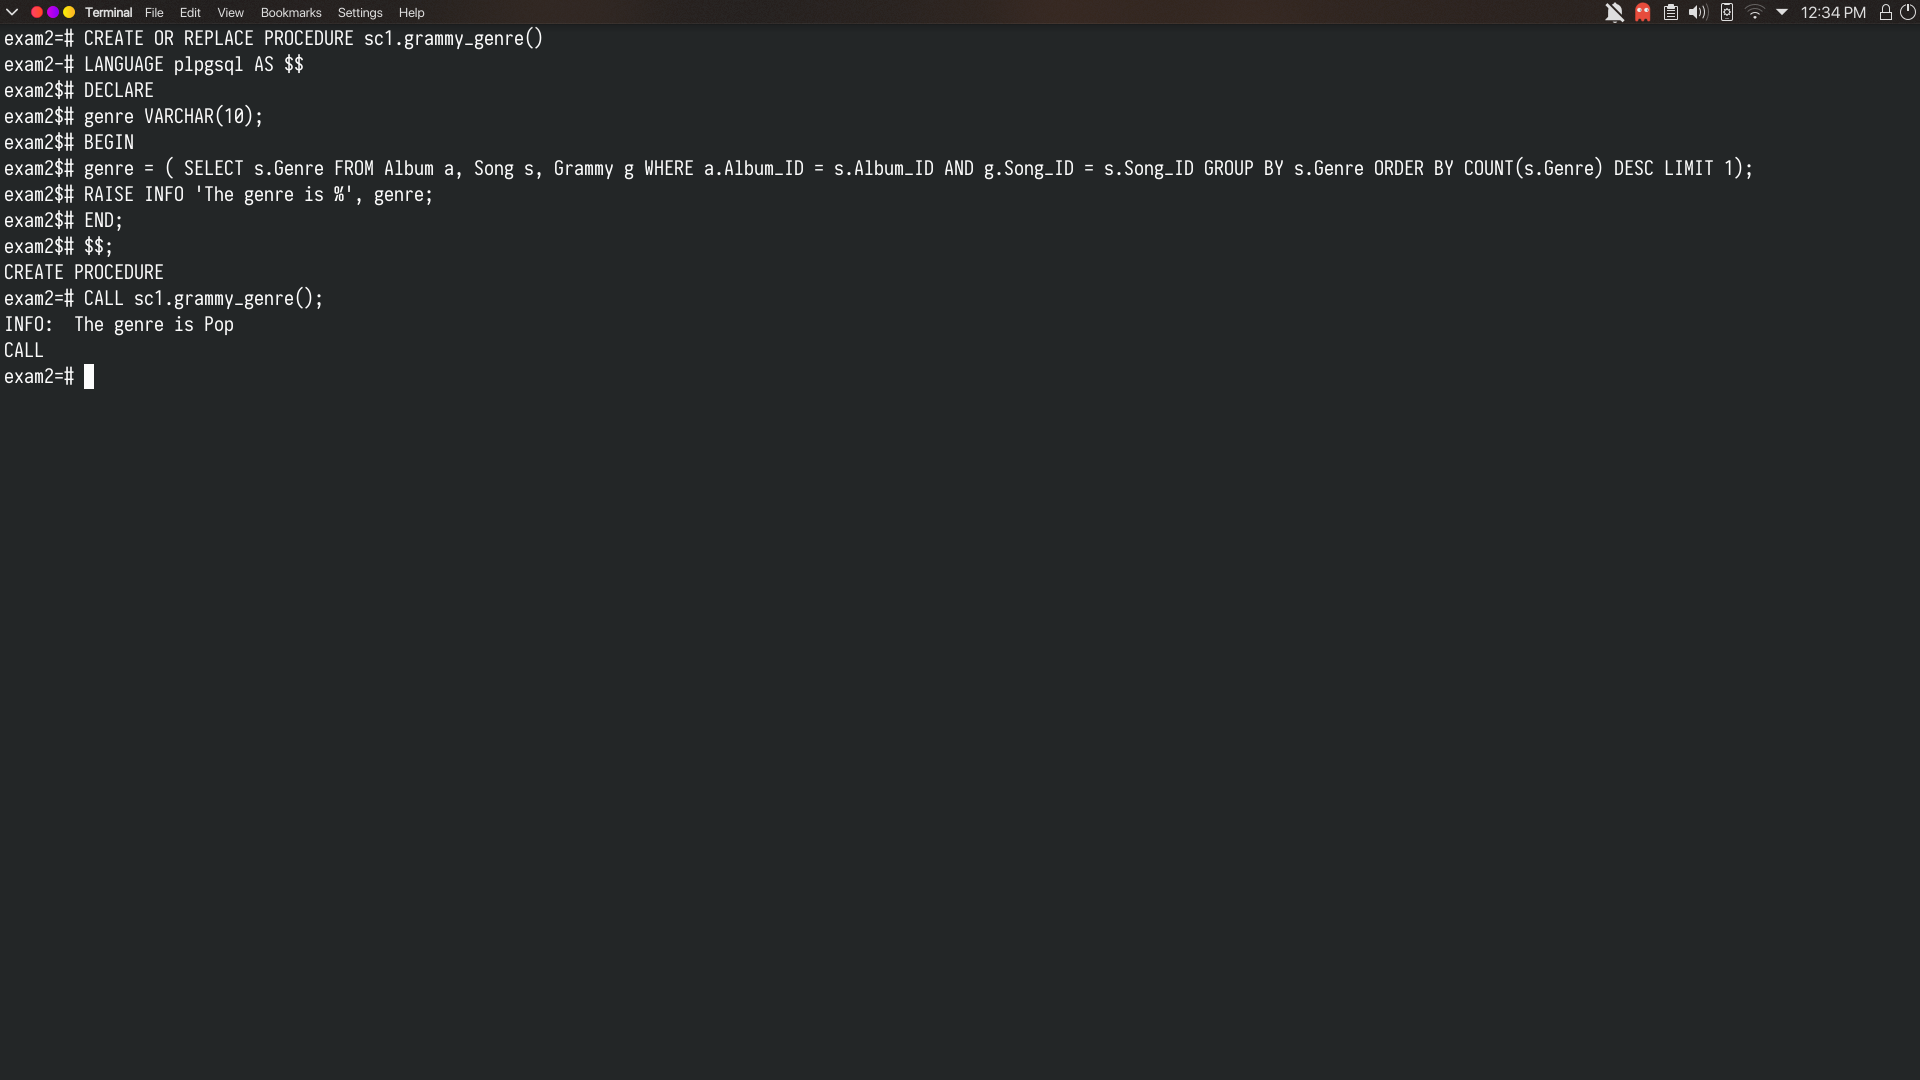
\includegraphics[width=\textwidth]{img/q/9.2.png}

\end{itemize}

\section*{Result}
Implemented the programs for the questions and their output is verified
\end{document} 